\chapter{Collision Detection}
\label{chapter:collision_detection}

\textbf{Author: Fabian Kleinrad} 

This chapter is going to concern itself with the method of detecting collisions within the path planning phase. The needed information about the environment stems from the data structures covered in chapter \ref{chapter:abstract_env}. 

\section{Fundamental Principle}
An essential part of autonomy in robotics is the aspect of collision avoidance. This is only possible if the robot has the means to identify and detect possible collisions and act suitably to circumvent collisions from happening.\newline
In Autumn this step of collision detection happens alongside with path planning. With the collision detection being a very cost intensive process it is important to optimize the algorithm for better performance, while simultaneously keeping a safety margin. This safety margin is especially important since the algorithm controls an UAV. 

\subsection{Base Algorithm}
The principle of the collision detection is very simple, due to the organized and semi organized data structures the algorithm works with. To check for collisions a function can be called that takes Cartesian coordinates as parameters and returns a value that indicates if an obstacle is present or not. All the collision detection algorithm has to do is to check if there are any collisions between two points sampled by the path planning algorithm. In order two accomplish this task the Bresenham's Algorithm will be used.\newline

\subsubsection{Bresenham's Algorithm} 
The Bresenham's Algorithm is a solution to the problem of rasterizing curves. Rasterizing being the process of converting a curves or lines into cells on a grid, representing the same shape. The Algorithm covers many different shapes, but because of the nature of the path planning algorithm used only a straight line will be necessary.\newline
The algorithm works by calculating an error for each candidate cell. The formula for this error being: $e=(y-y_0)dx-(x-x_0)dy$. Hereby $x$ and $y$ are the coordinates of the cell the error is calculated for, which are being subtracted by the coordinates of the starting point. $dx$ and $dy$ are the differences between the first and last point of the line. By calculating the errors for each cell, it is made possible to choose cells best representing the original line.\footcite{Zingl2012}

\begin{figure}[h]
	\centering
	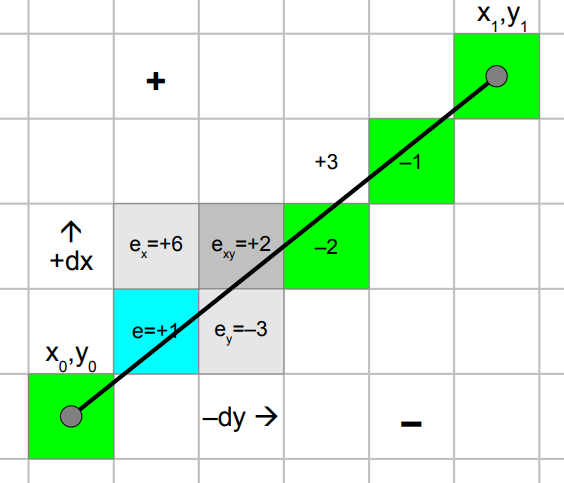
\includegraphics[width=0.5\linewidth]{img/Bresenhams}
	\caption{Application of Bresenham's Algorithm to a straight line, with visible errors. \cite{Zingl2012}}
	\label{fig:collision_detection_bresenham}
\end{figure}

\section{Implementation}

\subsection{2 dimensional space}

\subsection{3 dimensional space}

